\chapter{Automated Vulnerability Analysis of Smart Contracts on Ethereum} 
\label{ch:Slither-simil}

\section{Introductory Remarks}
With the rapid growth of blockchains, market contracts—universal and essential software applications—have attracted growing attention.
On the Ethereum Mainnet, for instance, more than ten million smart contracts have been installed.

An event-driven, self-executing, state-based software known as a "smart contract" is created using high-level programming languages like Vyper and Solidity.
In order to facilitate quick and reliable transactions, smart contracts have been widely implemented in various business fields.

Because of their distinct features, smart contracts require more work to build than standard programs do.
First, compared to regular programs, smart contracts are more prone to bugs.
A smart contract that has been published cannot be changed because "code is law."
This is because smart contract transactions always include cryptocurrencies, each worth millions of dollars (e.g., The DAO).
A smart contract bug could cause a substantial loss.
Therefore, it is essential to check contracts for accuracy before releasing them.
This necessitates the reuse of earlier contract development experience when creating new contracts.
The creation and upkeep of smart contracts can be made much easier by using program mining techniques for smart contracts like summarization, checking, and code search.
The conventional statistical analysis tools for detecting weaknesses in smart contracts purely rely on manually defined patterns, which are likely to be error-prone and can cause them to fail in complex situations.
Expert attackers can, therefore, quickly exploit these manual inspection patterns.
To minimize the risk of attackers, machine learning-powered systems provide more secure solutions relative to hard-coded static checking tools.

Surucu et al.~\cite{surucu2022survey} provide the first-ever survey on machine learning methods utilized to discover and mitigate vulnerabilities in smart contracts.
In order to set the ground for further development of ML methods on smart contract vulnerability detection, They reviewed many ML-driven intelligent detection mechanisms on the following databases:
Google Scholar, Engineering Village, Springer, Web of Science, Academic Search Premier, and Scholars Portal Journal.
Based on their survey paper, we briefly go over the existing analysis tool first and then the novel deep-learning-based methodologies proposed in the literature over the past few years
in chronological order, and we add some of the works missing in ~\cite{surucu2022survey} as well and update the list.
Afterward, we propose our solution, \slithersimil, and how it led us to the development of \etherbase.


\section{Traditional Security Analysis Methods in Smart Contracts}

Classic software testing technologies applied toward smart contract security analysis can be divided into three categories;

In the following, we will go over the tools proposed from the perspective of the technology they employ to tackle the smart contract security problem;
Ren et al.~\cite{Empirical-Evaluation-of-Smart-Contract-Testing:What-is-the-Best-Choice} provides three broad categories of tools based on their utilized methodology,
namely Static Analysis, Dynamic Fuzzing, and Symbolic Execution.

Using the static analysis method, we can analyze the program at both the source code (high-level) and bytecode (low-level) scopes before conducting any runtime execution.
Static analysis-based tools can scan a whole code base, but they also generate a lot of false positives as a result of their scans.
There are normally three main stages to a static analysis process:
\begin{itemize}
  \item building an intermediate representation (IR), such as abstract syntax tree (AST) for a deeper analysis compared to analyzing the raw text/source code;
  \item complementing the generated IR with additional metadata with methods such as control flow, data flow analysis, and symbolic execution.
  \item vulnerability detection w.r.t. a database of patterns and specific threshold defines vulnerability criteria.
\end{itemize}
Tools that leverage the static analysis methods typically convert the raw form of the input program into an intermediate representation and then perform a series of analyses on those representations based on a pre-defined database of vulnerability patterns and filter out the suspicious snippets of the input program.
Slither~\cite{slither}, Securify~\cite{securify}, and SmartCheck~\cite{securify} are categorised as instances of static analyzers.

Fuzzing~\cite{chen2018systematic} is a technique for finding software bugs that involve creating erroneous input data and watching the target program's unusual output while it runs.
It allows developers to generate exploits for security-critical programs and ensure a uniform standard of quality through prepared tests but does not narrow down the causes of detected bugs.
A fuzzing engine will first try to generate initial seeds to form executable transactions when applied to smart contracts. Regarding the feedback on test results,
it will dynamically adjust the generated data to explore as much smart contract state space as possible.
Finally, it will analyze the status of each transaction based on the finite state machine to detect whether there is an attackable threat.
ContractFuzzer~\cite{contractfuzzer}, ReGuard~\cite{liu2018reguard}, and sFuzz~\cite{nguyen2020sfuzz} are among the modt cited smart contract fuzzers.

Symbolic execution is a technique for finding software bugs that involve creating symbolic values and watching the target program's unusual output while it runs.
When using symbolic execution to analyze a program, it will use symbolic values as input instead of the specific values during the execution.
Tools leveraging this technique explore a state space with a high degree of semantic awareness.~\cite{boyer1975select}
Symbolic execution can simultaneously explore multiple paths the program can take under different inputs, but it also faces unavoidable problems such as path explosion.~\cite{Empirical-Evaluation-of-Smart-Contract-Testing:What-is-the-Best-Choice}
The symbolic execution tools usually build a control flow graph based on the Solidity bytecode of the smart contracts being tested.
Afterward, they implement constraints based on the characteristics of smart contract vulnerabilities and finally use the constraint solver to generate satisfying test cases.
Oyente~\cite{oyente}, Mythril~\cite{mythril}, and Manticore~\cite{mossberg2019manticore} support symbolic execution for smart contracts.


\section{Deep Learning in Smart Contracts} \label{sec:dl-models}

In this section, we will go over some of the literature focusing their efforts on replacing the existing tools' capabilities explained in the previous section with machine learning-based techniques.
Afterward, we will go over the tool we developed, \slithersimil.

There have been many efforts focused on utilizing ML-based techniques in the field of vulnerability discovery and mitigation with a specific focus on the programming language Solidity and
its lower-level representations.

While existing symbolic tools (like Oyente) for assessing vulnerabilities have shown to be effective, Goswami et al. said in 2018 that their execution time grows noticeably with the depth of invocations in a smart contract (cite: Grech2019GigaHorse).
They suggested an LSTM neural network model find flaws in ERC-20 smart contracts to create a quicker and more effective replacement for symbolic analysis tools.
This paper's preprocessing procedures were remarkably similar to those employed by~\cite{madmax}.
A dataset of 165,652 ERC-20 smart contracts was used for training and testing the model, and it contained bytecode data that Maian and Mythril had annotated (statistical code analysis tools).
On the testing set, the proposed model had an F1 score of 93.26%, 93.26 percent accuracy, and 92 percent recall.
Additionally, they have contrasted the time performance of their model with that of Maian and Mythril's symbolic analysis tools (static analysis tools).
Their suggested model operated on a test set of 5,000 random tokens in 15 seconds, while Maian and Mythril needed 32,476 and 9,475 seconds, respectively.
These findings show a similar advancement over symbolic analysis methods to that shown in citegrech2019gigahorse.

To identify security concerns to smart contracts in 2018, Liao et al. used a sequence learning approach (cite: madmax).
The Ethereum blockchain dataset from Google Big Query was used to acquire smart contract data.
Ultimately, 620,000 contracts from this source were used to train an LSTM model. Once more, one-hot vectors were used to represent the derived opcodes from the contracts.
These vectors were converted into code vectors using embedding methods, resulting in decreased dimensionality and a stronger capability to capture potential relationships between sequences because this representation produces highly sparse and uninformative features.
The statistical characteristics of the opcode lengths of contracts determined to be vulnerable and safe have been compared as another stage in the preprocessing process.
They decided to only include contracts with a maximum opcode length of 1600 since they noticed that the features of the two categories varied noticeably.
Additionally, it was discovered that the dataset's distribution (as labeled by MAIAN) was unbalanced, with non-vulnerable cases making up 99.03 percent of the dataset.
In order to obtain a fair distribution in the training set, all vulnerable contracts were clustered together and oversampled using the Synthetic Minority Oversampling Technique (SMOTE).
The outcomes showed that sequential learning methods outperformed symbolic analysis tools.
The model earned an F1 score of 86.04 percent and a vulnerability detection accuracy of 99.57 percent.

To improve the vulnerability identification of smart contracts, citeetehrTrust in 2019 presented the SoliAudit concept.
Solidity's smart contract source code is transformed into an opcode sequence to maintain the execution structure.
Each contract is run via a vulnerability scanner and a dynamic fuzzer.
The fuzzer (this term was introduced in an earlier paper) will parse the Application Binary Interface (ABI) of a smart contract to extract its declared function descriptions, data types of their arguments, and their signatures, whereas the vulnerability analyzer consists of a static machine learning classifier, which detects vulnerable classes.
The detected vulnerable smart contract inputs and functions will then be returned.
The creators of citeetehrTrust proposed the concept of a smart contract fuzzer.
Thirteen vulnerabilities were identified by a vulnerability analyst using a set of labels produced by analytical tools like Oyente and Remix.
Before utilizing these labels to train the opcode sequence data, two different feature extraction techniques were examined. These included word2vec and n-gram with tf-idf.
The studies were conducted using the above-mentioned approach and techniques, including Gradient Boosting, Support Vector Machine, K-Nearest Neighbor, Decision Trees, Random Forests, and Logistic Regression.
A matrix was produced by the latter (word2vec), and a convolutional neural network (CNN) was chosen to train it since it considers the matrix's internal structure.
However, the results of this feature extraction and training combination were subpar.
With an accuracy rate of 97.3 percent and an F1 score of 90.4 percent, Logistic Regression produced the best results for categorizing vulnerabilities.

In 2019, In this research, we proposed a machine learning-based
model to detect security vulnerabilities of smart contracts
on the Ethereum platform. We used static code analysis as
the underlying technology and trained various machine
learning models for security vulnerabilities. Our
model found 16 different vulnerabilities with an
average accuracy of 95%. Our approach significantly improved computational time and resources compared
to directly using static code analysis tools. Checking many smart contracts using different static code analyzers
is a huge burden on developers. In addition, they need to learn
how each analyzer works and combine the results for a full
evaluation. Furthermore, our model can be used to identify
security vulnerabilities parallel to the development process
of smart contracts, thus decreasing the cost of development
by preventing the security vulnerabilities from being introduced
in the early stages. Our proposed model also applies to
other languages and platforms since the model has no language
or platform dependencies. Training the model
with different attentive language datasets and choosing
the corresponding static code analyzers and AST builders,
new machine learning code analyzers can be generated by
following the steps described in Section III.

In 2020, Xing et al. ~\cite{xing2020new} proposed a feature extraction method named slicing matrix.
It consists of segmenting the opcode sequences derived from
smart contract bytecodes to extract opcode features from each one individually.
The purpose of this segmentation is to separate useful and useless opcodes.
The extracted opcode features are then combined to form the slice matrix.
To carry out a comparative analysis, three models were created.
These were namely Neural Network Based on opcode Feature (NNBOOF), Convolution Neural Network Based on Slice Matrix (CNNBOSM), Random Forest Based on opcode Feature
(RFBOOF) ~\cite{hu2021comprehensive}.
These models were each tested on three different vulnerability classification tasks: greedy contract vulnerability, arithmetic overflow/underflow vulnerability, and short address vulnerability.
While RFBOOF achieved the best results in all three cases based on precision, recall, and F1 evaluation metrics, CNNBOSM performed slightly better than NNBOOF.
The authors mention that the slice matrix feature needs further exploring.

In 2020, Ethereum established itself as a popular platform for facilitating safe, Blockchain-based financial and commercial transactions.
However, the security of Ethereum's smart contracts is a significant issue.
Numerous discovered flaws and weaknesses in smart contracts not only complicate the upkeep of the blockchain but also result in significant financial losses. Better tools are needed to help developers verify smart contracts and ensure their dependability.
In this article, we suggest SMARTEMBED, a web service tool that can assist Solidity developers in identifying repeated contract code and clone-related problems in smart contracts.
Our technology is based on methods for comparing codes and code embeddings.
We can effectively identify code clones and clone-related bugs for any solidity code provided by users, which can help to increase the users' confidence in the reliability of their code. We do this by comparing the similarities between the code embedding vectors for existing solidity code in the Ethereum blockchain and known bugs.
SMARTEMBED can be used for studies of smart contracts on a large scale in addition to uses by specific developers.
We discovered that solidity code has a substantially higher clone ratio than traditional software when applied to more than 22K contracts taken from the Ethereum blockchain. Based on our modest bug database, 194 clone-related defects can be efficiently and effectively diagnosed with a precision of 96%.


To identify various smart contract vulnerabilities, Liu Z. et al. designed a machine learning approach combining GNN and expert knowledge (cite:hwang2020gap).
The goal of a graph neural network (GNN), a deep learning technique, is to make inferences from data represented by graphs.
A graph is a data structure used in computer science that consists of nodes (also known as vertices) and edges. According to research, the semantic relationships between programming elements can be preserved when written programs are transformed into symbolic graph representations.
As a result, contract graphs can be used to represent smart contract codes.
The suggested strategy, as depicted in figure 3, begins with two distinct concurrent processes (Security pattern extraction and contract graph extraction) and then uses a combining layer to combine patterns in each segment to identify vulnerabilities.
A feed-forward neural network first creates the pattern feature for extracting security patterns from the contract's source code.
To extract the expert patterns from smart contract functions, they employed an open-source program.
A GNN must be created in the second process (message propagation phase) to produce a contract graph.
Nodes, or program elements, made up the GNN model, while edges, or the next function to be executed, indicated the flow of each program element.
Later, using a node elimination approach, undesirable nodes and edges are eliminated.
The authors used a preprocessing technique that involved casting the source code's extensive control and data flow semantics into a contract graph.
Following this, they created a node elimination stage to normalize the network and highlight important nodes.
The vulnerability detection phase, where both extracted features are integrated with convolution and a fully connected layer, was used to combine these two simultaneous procedures.
The suggested model is tested against security detection methods that are not ML-based, including Oyente, Mythril, Smartcheck, Securify, and Slither.
Re-entrancy, timestamp dependence, and endless loop vulnerabilities of each function in the source code were all searched for by each algorithm and the proposed model.
a
The proposed methods (CGE) found reentrancy and timestamp-dependent type vulnerabilities with an accuracy of 89 percent and an infinite loop vulnerability (cite:hwang2020gap) with an accuracy of 83 percent.


When a piece of code is rewritten, the Eth2Vec model is suggested to address a flaw in the present vulnerability detection tools. A code rewrite in a programming language is reimplementing a source code's functionality without utilizing the original.
Finding vulnerabilities becomes more difficult when the smart contract codes are modified.
The authors first transformed each smart contract's source code into EVM bytecodes.
Only useful information (such as function ids and lists of callee functions) for vulnerability detection was taken out of the bytecode by the authors.
A neural network structure is utilized as the final step to find any vulnerabilities in the source code.
Five hundred contracts were used to test the suggested model, and even though the contracts were changed, the Eth2Vec model could identify vulnerabilities with a 77 percent accuracy.

O. Lutz et al.~\cite{Dolan2016lava} and present another technique for identifying weaknesses in smart contracts.
The authors offer a method called ESCORT, which employs a Deep Neural Network model to discover the semantics of the input smart contract and identify particular vulnerability types based on the discovered semantics.
The ESCORT model aims to get over the limitations of existing non-DNN models in terms of scalability and generalization.
With a detection period of 0.02 seconds for each contract, the experimental results of this article produced an F1 accuracy score of 9 percent on six different vulnerability types.
Scalability is easier to achieve with rapid detection times, which meets one of the author's objectives.
The ESCORT model, therefore, somewhat resolves the problems identified in earlier works, such as Y. Xu or N. Lesimple's models, where the model can realize novel weaknesses.~\cite{grech2019gigahorse}
Unfortunately, it is relatively challenging to derive interpretability from such models, and even if new vulnerabilities are discovered, figuring out their root causes is still very challenging.
Sun et al. used machine learning to try and find the following vulnerabilities: reentrancy, arithmetic problems (integer overflow/underflow), and timestamp dependencies.
In order to accommodate for differences in instructions between compilers, some stack operating instructions were trimmed into more general versions (e.g., SWAP1, SWAP2,..., SWAPn. SWAPx).
After that, as a label normalization step, opcodes were divided into nine categories depending on their purposes.
A word2vec transformation of the opcode sequences prior to the convolutional layers was carried out, just like in "cite" etehrTrust.
This article introduces an additional self-attention layer in addition to the pooling and softmax layers that typically follow convolutional layers.
The one-hot encoders used to encode each opcode instruction are merely representatives and do not capture any functional similarity between them; therefore, the self-attention layer's goal is to establish a connection between adjacent words in the acquired feature matrix. ~\cite{grech2019gigahorse}.
By using self-attention, the word embedding process has been improved as a result.
CiteetehrTrust and this paper used CNNs to find vulnerabilities, but CiteetehrTrust used a word2vec embedding, whereas this paper used an attention method, which is why they got superior results. The key advantage of the newly developed model over the static analyzers that are already in use, such as Oyente and Mythril, is that it can attain comparable performance in a lot less time.
In their paper, Y. Xu et al. developed two unique methods for identifying vulnerable smart contracts: the Stochastic Gradient Descent (SGD) model and the K Nearest Neighbors (KNN) model.
They seek to use each machine learning model to discover eight of the most widely known classical vulnerability types, including arithmetic, reentrancy, denial of service, uncontrolled low-level calls, access control, faulty randomization, front running, and denial of service.
Similar to N.Lesimple's paper~\cite{he2019learning}, their model employs an AST structure as its input, enabling it to parse the smart contract code line by line.
Through the use of conventional techniques, the labels for the vulnerabilities were found.
High recall, precision, and accuracy are noted for four of the eight vulnerabilities in the paper.
The results for the remaining four were deemed inconclusive since there were not enough samples in the dataset.
The test set was produced from the outcomes of utilizing conventional approaches, similar to the N. Lesimple study, showing that the authors could not demonstrate how the KNN model differed from conventional methods.

In 2021, by using bigram properties from the streamlined operation codes of smart contracts, Wang et al. ~\cite{wang2020contractward} introduced their approach, ContractWard, to identify vulnerabilities in smart contracts.
They gathered a dataset of 49,502 smart contracts from the Etherscan website, verified before September 2018, and found that each contract had six potential weaknesses:
Integer overflow/underflow, transaction ordering dependency, call stack depth attack, timestamp dependency, and re-entrancy
Each smart contract's source code is converted to opcodes; A smart contract typically has 100 different opcodes and 4364 opcode components.
There were only 50 opcode types left after they conducted a simplifying process.
As a result, the authors grouped several opcodes with related functionality into a single category, which simplified the dataset's features.
Because they believe that operations have a stronger relationship with their neighbors, they later adopted the n-gram approach (a sliding window of binary-byte size) to track relationships between each opcode.
Each of the contract's many labels was assigned using the Oyente~\cite{oyente} system.
Due to the scarcity of particular vulnerabilities, the researchers ran into a class-imbalance problem after the labeling process.
Extreme Gradient Boosting (XGBoost), Adaptive Boosting (AdaBoost), Random Forest (RF), Support Vector Machine (SVM), and k-Nearest Neighbour were the five candidate ML models used in the training procedure (KNN).
By reaching above 96 percent F1, Micro-F1, and Macro-F1score, the XGBoost model demonstrated strong performance.

In 2022, Yuqi Fan et al. note that most of the studies on methods of vulnerability detection regarding smart contracts take rely on pre-defined manual rules from experts and auditing professionals.~\cite{fan2021smart}
Devising such rules and patterns are very time-intensive and labor-demanding.
They discuss the previous efforts at employing deep learning methods to make up for such shortcomings, but they fail to represent the source code/bytecode well semantically and structurally.
Then, they propose a novel model of Dual Attention Graph Convolutional Network (DA-GCN) to detect smart contract vulnerabilities.
They extract both control flow graph and opcode sequence from smart contracts' bytecodes and feed them as input into a feature extraction pipeline. Afterward, they use a multilayer neural network to identify the vulnerable smart contracts.
They tested their proposed model on smart contracts containing one of the two vulnerabilities: reentrancy and timestamp dependency.
Their experimental results demonstrated that the DA-GCN model achieved an accuracy of 91.2\% and 87.5\% in the two smart contract vulnerability detection tasks.

In 2022, Zhang et al. ~\cite{zhang2022novel} propose a novel model to detect smart contract vulnerabilities: ensemble learning (EL)-based contract vulnerability prediction method.
It is based on seven different neural networks using vulnerability data for vulnerability detection at the scope of smart contracts (single file-level scope).
Seven neural network (NN) models were first pre-trained using an information graph (IG) consisting of source datasets, which then were
integrated into an ensemble model called the Smart Contract Vulnerability Detection method based on
Information Graph and Ensemble Learning (SCVDIE). The effectiveness of the SCVDIE model was
verified using a target dataset composed of IG, and then its performances were compared with static
tools and seven independent data-driven methods. The verification and comparison results show that
the proposed SCVDIE method has higher accuracy and robustness than other data-driven methods
in predicting smart contract vulnerabilities.

Also, in 2022, Zhang et al.~\cite{zhang2022spcbig} propose another novel method for vulnerability detection:
A flexible and systematic hybrid model, which they have named the Serial-Parallel Convolutional Bidirectional Gated
Recurrent Network Model, incorporating Ensemble Classifiers (SPCBIG-EC).
Their new model shows noticeable improvements in performance concerning smart contract vulnerability detection.
In addition, they also propose a serial-parallel convolution (SPCNN) suitable for this hybrid model and generally serial combinatorial models.
It is equipped with the capability to extract features from an input sequence for multivariate combinations while retaining temporal structure and location information.
The Ensemble Classifier is used in the classification phase of the model to enhance its
robustness. In their experiments, they focused on six typical smart contract vulnerabilities and constructed two
datasets, CESC and UCESC, for multi-task vulnerability detection.
Numerous experiments showed that their proposal is better than most existing methods.
It achieved an F1-scores of 96.74\%, 91.62\%, and 95.00\% for reentrancy, timestamp
dependency, and infinite loop vulnerability detection.

\section{\slithersimil}

\textit{Parts of this section have been published in another piece~\cite{pilehchiha_2020} written by the same author of this dissertation and have been used here with permission.}

The efforts of security auditing companies like Trail of Bits, Inc. concerning automating smart contract security assessments have included works on an addition to an already prominent static analysis tool, Slither~\cite{slither}, to better help developers and researchers in their process of auditing smart contracts.

Trail of Bits, a prominent blockchain security firm, has manually curated a wealth of data—years of security assessment reports—and we decided to explore how to use this data to make the smart
contract auditing process more efficient with addition to Slither -a static analysis tool named \slithersimil.

Based on accumulated knowledge embedded in previous audits, we set out to detect similarly vulnerable code snippets in new clients' codebases.
Specifically, we explored machine learning (ML) approaches to automatically improve the performance of Slither, our static analyzer for Solidity, and facilitate the conduct of audits for auditors and general users.

Currently, human auditors with expert knowledge of Solidity and its security nuances scan and assess Solidity source code to discover vulnerabilities and potential threats at different granularity levels.
In our experiment, we explored how much we could automate security assessments to:
\begin{enumerate}
  \item Minimize the risk of recurring human error, i.e., the chance of overlooking known, recorded vulnerabilities.
  \item Help auditors sift through potential vulnerabilities faster and more easily while decreasing the rate of false positives.
\end{enumerate}

\slithersimil~\cite{slithersimil}, the statistical addition to Slither, is a code similarity measurement tool that uses state-of-the-art machine learning to detect similar Solidity functions.
When it began as an experiment last year under the codename crytic-pred, it was used to vectorize Solidity source code snippets and measure their similarity.
Last year, we took it to the next level and applied it directly to vulnerable code.

\slithersimil currently uses its representation of Solidity code, as introduced by~\cite{slither}, namely SlithIR.
SlithIR (Slither Intermediate Representation), to encode Solidity snippets at the granularity level of functions.
We thought the function-level analysis was a good place to start our research since
it is not too coarse (like the file level) and not too detailed (like the statement or line level).

As introduced by Feist et al., SlithIR was developed as an intermediate representation (IR) language with slither in mind to leverage it and represent Solidity code for further analysis.
Every smart contract written in Solidity can be decomposed into a control flow graph. Each node can contain up to a single Solidity expression in that graph, which is converted to a set of SlithIR instructions.
This representation makes implementing analyses easier without losing the critical semantic information contained in the Solidity source code.~\cite{slither}
SlithIR has a database of about 40 instruction expressions.
It has no internal control flow representation and relies on Slither's control-flow graph structure (SlithIR code is associated with each node in the graph).
The complete descriptions are available at~\cite{slithir}.

\begin{figure}
  \centering
  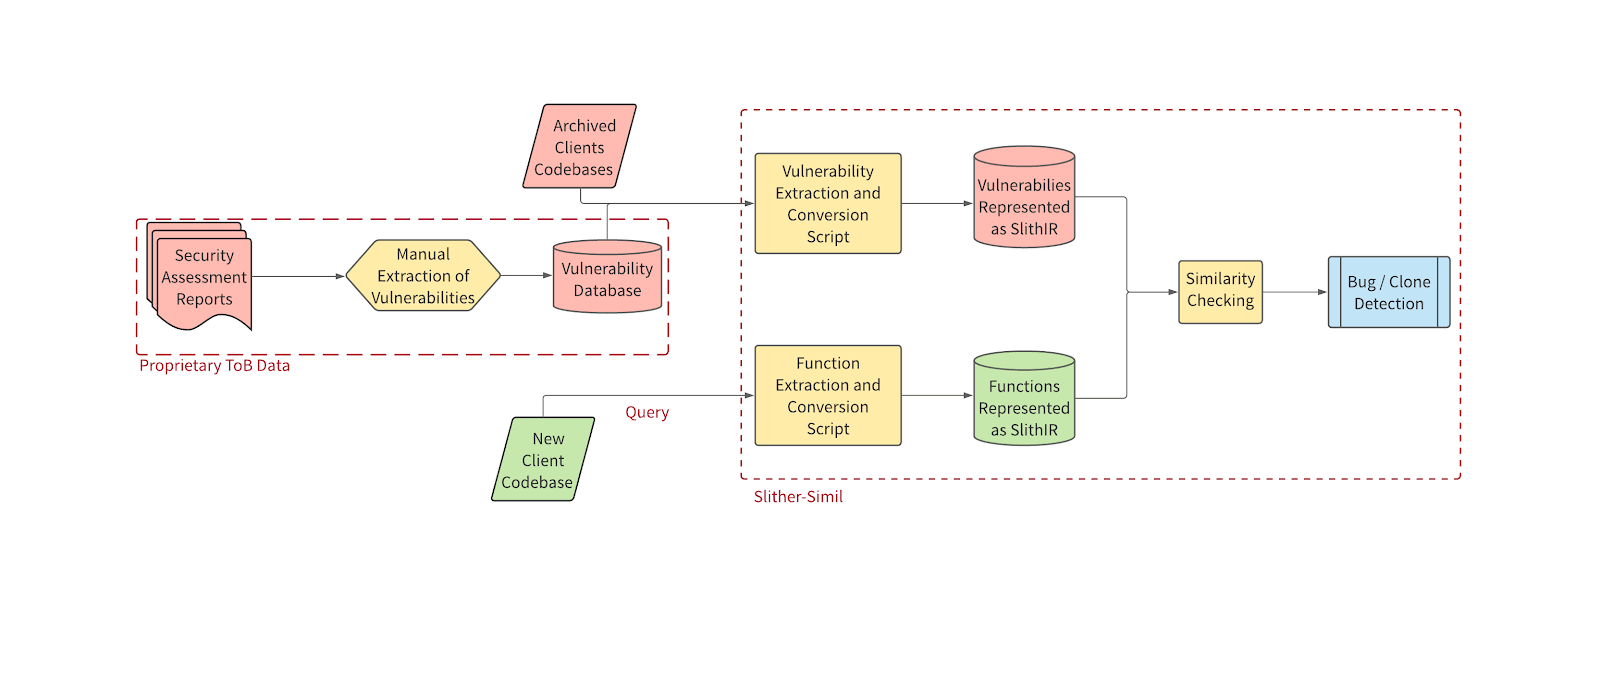
\includegraphics[width=\textwidth]{figures/slitherS.png}
  \caption{A high-level view of the process workflow of Slither-simil.}
  \label{fig:slithersimilhighlevel}
\end{figure}

In the process workflow of Slither-simil, we first manually collected vulnerabilities from the previous archived security assessments and transferred them to a vulnerability database.
Note that these are the vulnerabilities auditors had to find with no automation.

After that, we compiled previous clients' codebases and matched the functions they contained with our vulnerability database via an automated function extraction and normalization script.
By the end of this process, our vulnerabilities were normalized SlithIR tokens as input to our ML system.

Here is how we used Slither to transform a Solidity function to the intermediate representation SlithIR, then further tokenized and normalized it to be an input to \slithersimil:

\begin{lstlisting}[float,caption= complete Solidity function from the contract TurtleToken.sol., escapechar=\%, language=Solidity, label=lst:solidity-bug]
  function transferFrom(address _from, address _to, uint256 _value) public returns (bool success) {
        require(_value <= allowance[_from][msg.sender]);     // Check allowance
        allowance[_from][msg.sender] -= _value;
        _transfer(_from, _to, _value);
        return true;
  }
  \end{lstlisting}

  \begin{lstlisting}[float,caption= The same function with its SlithIR expressions printed out., escapechar=\%, language=Solidity, label=lst:solidity-bug]
Function TurtleToken.transferFrom(address,address,uint256) (*)
 
 
Solidity Expression: require(bool)(_value <= allowance[_from][msg.sender])
SlithIR: 
         REF_10(mapping(address => uint256)) ->    allowance[_from]
         REF_11(uint256) -> REF_10[msg.sender]
         TMP_16(bool) = _value <= REF_11
         TMP_17 = SOLIDITY_CALL require(bool)(TMP_16)
 
 
Solidity Expression: allowance[_from][msg.sender] -= _value
SlithIR: 
         REF_12(mapping(address => uint256)) -> allowance[_from]
         REF_13(uint256) -> REF_12[msg.sender]
         REF_13(-> allowance) = REF_13 - _value
 
 
Solidity Expression: _transfer(_from,_to,_value)
SlithIR: 
         INTERNAL_CALL,      TurtleToken._transfer(address,address,uint256)(_from,_to,_value)
 
 
Solidity Expression: true
SlithIR: 
         RETURN True
    \end{lstlisting}


First, we converted every statement or expression into its SlithIR correspondent, then tokenized the SlithIR sub-expressions and further normalized them so more similar matches would occur
despite superficial differences between the tokens of this function and the vulnerability database.

\begin{lstlisting}[float,caption= Normalized SlithIR tokens of the previous expressions., escapechar=\%, language=Solidity, label=lst:solidity-bug]
type_conversion(uint256)
 
binary(**)
 
binary(*)
 
(state_solc_variable(uint256)):=(temporary_variable(uint256))
 
index(uint256)
 
(reference(uint256)):=(state_solc_variable(uint256))
 
(state_solc_variable(string)):=(local_solc_variable(memory, string))
 
(state_solc_variable(string)):=(local_solc_variable(memory, string))
 
...
  \end{lstlisting}

After obtaining the final form of token representations for this function, we compared its structure to that of the vulnerable functions in our vulnerability database.
Due to the modularity of Slither-simil, we used various ML architectures to measure the similarity between any number of functions.

Let us take a look at the function transferFrom from the ETQuality.sol smart contract to see how its structure resembles our query function:

Comparing the statements in the two functions, we can easily see that they both contain, in the same order, a binary comparison operation (>= and <=), the same type of operand comparison, and another similar assignment operation with an internal call statement and an instance of returning a "true" value.

As the similarity score goes lower towards 0, these sorts of structural similarities are observed less often and in the other direction; the two functions become more identical, so the two
functions with a similarity score of 1.0 are identical to each other.

Research on automatic vulnerability discovery in Solidity has taken off in the past two years, and tools like Vulcan~\cite{srikant2020vulcan} and SmartEmbed~\cite{gao2019smartembed},
which use ML approaches to discovering vulnerabilities in
smart contracts are gradually showing promising results, with fewer false positives in specific vulnerability reports.

However, all the current related approaches focus on vulnerabilities already detectable by static analyzers like Slither and Mythril, while our experiment focused on the vulnerabilities these
tools were not able to identify—specifically, those undetected by Slither.

Much of the academic research of the past five years has focused on taking ML concepts (usually from the field of natural language processing) and using them in a development or code analysis context,
typically referred to as code intelligence.
Based on previous related work in this research area, we aim to bridge the semantic gap between the performance of a human auditor and an ML detection system to discover vulnerabilities, thus
complementing the work of Trail of Bits human auditors with automated approaches (i.e., Machine Programming, or MP~\cite{gottschlich2018three}).

We still face the challenge of data scarcity concerning the scale of smart contracts available for analysis and the frequency of interesting vulnerabilities appearing in them.
We can focus on the ML model because it is a more facilitated process, but it does not do much good for us in the case of Solidity, where even the language itself is very young, and we need to
tread carefully in how we treat the amount of data we have at our disposal.
Archiving previous client data was a job since we had to deal with the different solc versions to compile each project separately.

This past summer, we resumed the development of Slither-simil and SlithIR with two goals in mind:
Research purposes, i.e., the development of end-to-end similarity systems lacking feature engineering.
Practical purposes, i.e., adding specificity to increase precision and recall.
We implemented the baseline text-based model with FastText to be compared with an improved model with a tangibly significant difference in results;
e.g., one not working on software complexity metrics, but focusing solely on graph-based models, as they are the most promising ones right now.

For this, we have proposed several techniques to try out with the Solidity language at the highest abstraction level, namely, source code.

To develop ML models, we considered both supervised and unsupervised learning methods.
First, we developed an unsupervised baseline model based on tokenizing source code functions and embedding them in a Euclidean space.
(Figure 8) to measure and quantify the distance (i.e., dissimilarity) between different tokens.
Since functions are constituted from tokens, we just added the differences to get the (dis)similarity between any two different snippets of any size.

The diagram below shows the SlithIR tokens from a set of training Solidity data spherized in a three-dimensional Euclidean space, with similar tokens closer to each other in vector distance.
Each purple dot shows one token.

We are developing a proprietary database of our previous clients and their publicly available vulnerable smart contracts and references in papers and other audits.
Together they will form one unified, comprehensive database of Solidity vulnerabilities for queries, later training, and testing newer models.

We are also working on other unsupervised and supervised models, using data labeled by static analyzers like Slither and Mythril.
We are examining deep learning models with much more expressivity we can model source code with—specifically, graph-based models, utilizing abstract syntax trees and control flow graphs.

Furthermore, we are looking forward to checking out the performance \slithersimil on new audit tasks to see how
it improves our assurance team's productivity (e.g., in triaging and finding the low-hanging fruit more quickly).
We will also test it on Mainnet when it becomes more mature and automatically scalable.

\slithersimil~ is now available on Github and ready to use.
For end users, it is the simplest CLI tool available:
The user can input one or multiple smart contract files (either directory, .zip file, or a single .sol).
Identify a pre-trained model, or separately train a model on a reasonable amount of smart contracts.

\section{Concluding Remarks}

In this chapter, we went over the research community's efforts to propose machine-learning-based methods to discover and mitigate vulnerabilities in smart contracts compared to the existing approaches used in the industry.
We also went over \slithersimil, a powerful tool with the potential to measure the similarity between function snippets of any size written in Solidity.
We are continuing to develop it, and based on current results and recent related research, we hope to see impactful real-world results before the end of the year.
Nevertheless, there is a lacking here, and that is the bottleneck of datasets that help us train and test bigger and more comprehensive models.
In the next chapter we will introduce \etherbase and how the development of \slithersimil~has extended into the development of \etherbase as a solution for us and the broader research community.